\documentclass[tikz,border=8pt]{standalone}
% Shared look for every TikZ diagram. Load with % Shared look for every TikZ diagram. Load with % Shared look for every TikZ diagram. Load with \input{../../tools/tikz-style.tex}
\usepackage[T1]{fontenc}
\usepackage{lmodern}
\renewcommand{\sfdefault}{lmr}  % diagrams use the same serif as the text
\usetikzlibrary{arrows.meta, positioning, shapes.geometric, calc, fit, backgrounds}
\definecolor{cblue}{HTML}{4C78A8}
\definecolor{corange}{HTML}{F58518}
\definecolor{cgreen}{HTML}{54A24B}
\definecolor{cred}{HTML}{E45756}
\definecolor{cpurple}{HTML}{B279A2}
\definecolor{cgrey}{HTML}{6B6B6B}
\tikzset{
  every picture/.style={font=\sffamily, line width=1.2pt},
  box/.style={draw=#1, fill=#1!12, rounded corners=4pt, align=center, inner sep=7pt, minimum height=1.1cm},
  box/.default=cgrey,
  arrow/.style={-{Stealth[length=3mm]}, draw=cgrey, line width=1.4pt},
  title/.style={font=\sffamily\bfseries\Large},
  note/.style={font=\sffamily\small, text=cgrey, align=center},
}
\AtBeginDocument{\hyphenpenalty=10000 \exhyphenpenalty=10000}

\usepackage[T1]{fontenc}
\usepackage{lmodern}
\renewcommand{\sfdefault}{lmr}  % diagrams use the same serif as the text
\usetikzlibrary{arrows.meta, positioning, shapes.geometric, calc, fit, backgrounds}
\definecolor{cblue}{HTML}{4C78A8}
\definecolor{corange}{HTML}{F58518}
\definecolor{cgreen}{HTML}{54A24B}
\definecolor{cred}{HTML}{E45756}
\definecolor{cpurple}{HTML}{B279A2}
\definecolor{cgrey}{HTML}{6B6B6B}
\tikzset{
  every picture/.style={font=\sffamily, line width=1.2pt},
  box/.style={draw=#1, fill=#1!12, rounded corners=4pt, align=center, inner sep=7pt, minimum height=1.1cm},
  box/.default=cgrey,
  arrow/.style={-{Stealth[length=3mm]}, draw=cgrey, line width=1.4pt},
  title/.style={font=\sffamily\bfseries\Large},
  note/.style={font=\sffamily\small, text=cgrey, align=center},
}
\AtBeginDocument{\hyphenpenalty=10000 \exhyphenpenalty=10000}

\usepackage[T1]{fontenc}
\usepackage{lmodern}
\renewcommand{\sfdefault}{lmr}  % diagrams use the same serif as the text
\usetikzlibrary{arrows.meta, positioning, shapes.geometric, calc, fit, backgrounds}
\definecolor{cblue}{HTML}{4C78A8}
\definecolor{corange}{HTML}{F58518}
\definecolor{cgreen}{HTML}{54A24B}
\definecolor{cred}{HTML}{E45756}
\definecolor{cpurple}{HTML}{B279A2}
\definecolor{cgrey}{HTML}{6B6B6B}
\tikzset{
  every picture/.style={font=\sffamily, line width=1.2pt},
  box/.style={draw=#1, fill=#1!12, rounded corners=4pt, align=center, inner sep=7pt, minimum height=1.1cm},
  box/.default=cgrey,
  arrow/.style={-{Stealth[length=3mm]}, draw=cgrey, line width=1.4pt},
  title/.style={font=\sffamily\bfseries\Large},
  note/.style={font=\sffamily\small, text=cgrey, align=center},
}
\AtBeginDocument{\hyphenpenalty=10000 \exhyphenpenalty=10000}

\begin{document}
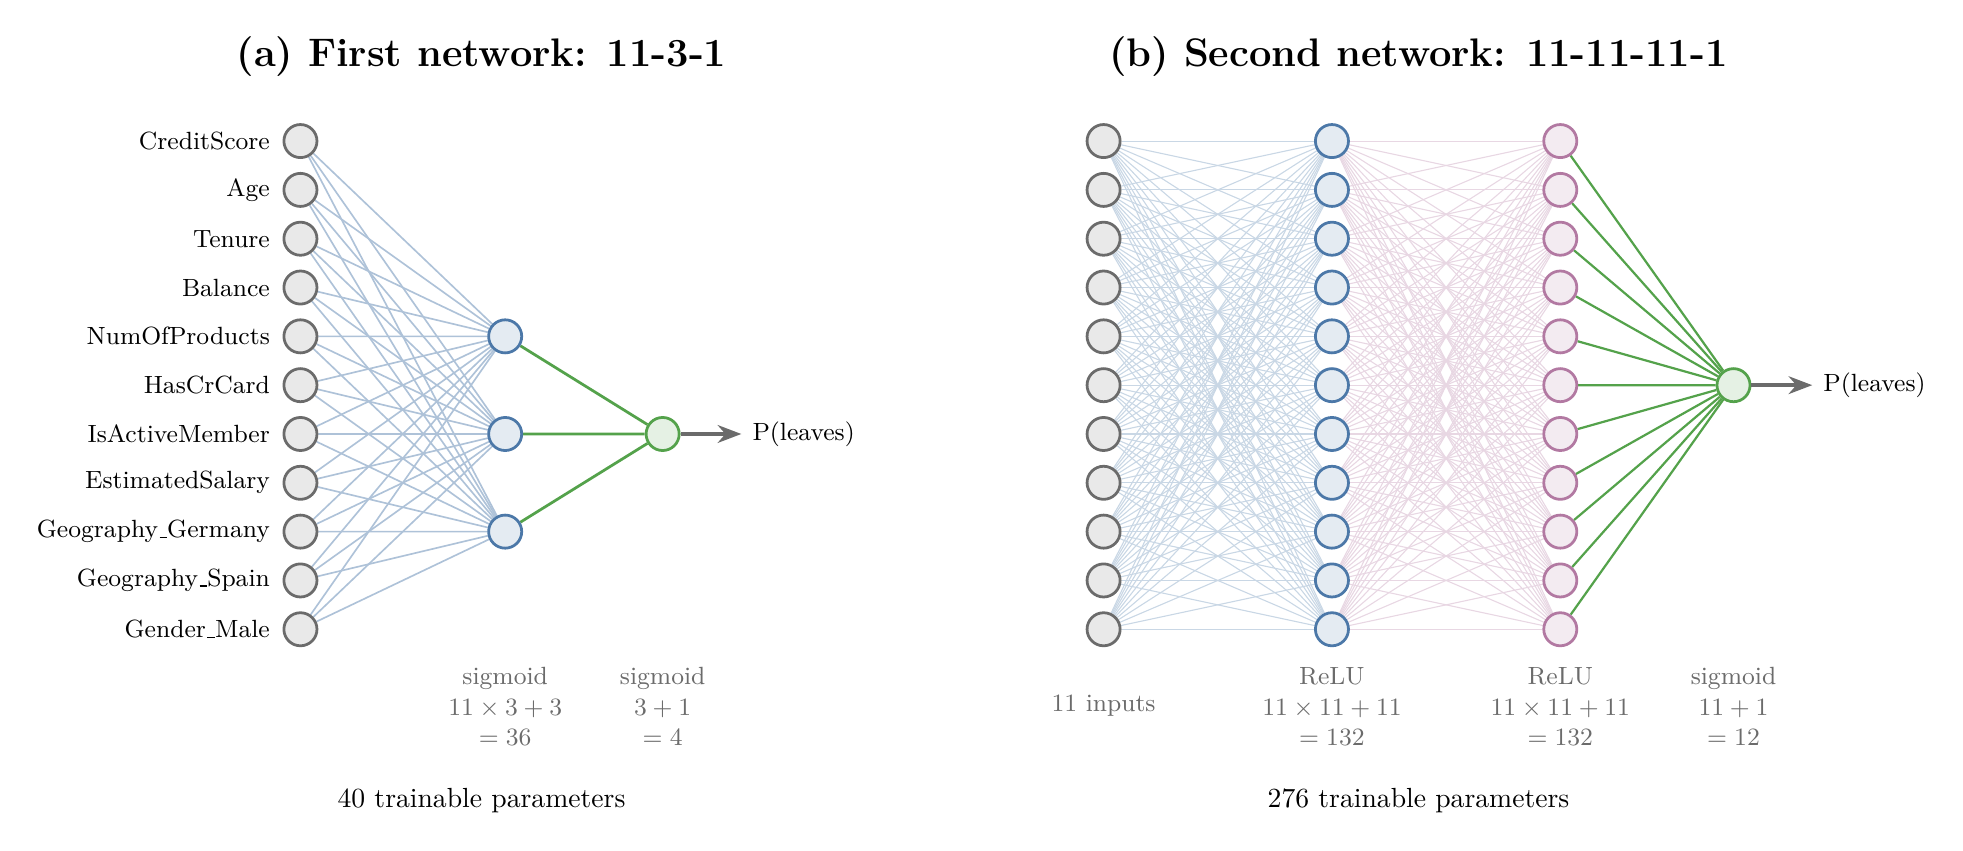
\begin{tikzpicture}[
  inp/.style={circle, draw=cgrey, fill=cgrey!15, minimum size=0.42cm, inner sep=0pt, line width=1pt},
  hid/.style={circle, draw=#1, fill=#1!15, minimum size=0.42cm, inner sep=0pt, line width=1pt},
  lab/.style={font=\sffamily\small, anchor=east}]
  % ---------- (a) first network: 11-3-1 ----------
  \foreach \n [count=\i] in {CreditScore, Age, Tenure, Balance, NumOfProducts, HasCrCard, IsActiveMember,
                              EstimatedSalary, Geography\_Germany, Geography\_Spain, Gender\_Male} {
    \node[inp] (a0\i) at (0, -0.62*\i) {};
    \node[lab] at (-0.25, -0.62*\i) {\n};
  }
  \foreach \j in {1,2,3} \node[hid=cblue] (a1\j) at (2.6, -1.86-1.24*\j) {};
  \node[hid=cgreen] (a2) at (4.6, -4.34) {};
  \begin{scope}[on background layer]
    \foreach \i in {1,...,11} \foreach \j in {1,2,3} \draw[cblue!45, line width=0.6pt] (a0\i) -- (a1\j);
    \foreach \j in {1,2,3} \draw[cgreen, line width=1pt] (a1\j) -- (a2);
  \end{scope}
  \draw[arrow] (a2) -- ++(1.0,0) node[right, align=left, font=\sffamily\small] {P(leaves)};
  \node[title] at (2.3, 0.45) {(a) First network: 11-3-1};
  \node[note] at (2.6, -7.8) {sigmoid\\$11 \times 3 + 3$\\$= 36$};
  \node[note] at (4.6, -7.8) {sigmoid\\$3 + 1$\\$= 4$};
  \node[font=\sffamily\normalsize] at (2.3, -9.0) {40 trainable parameters};
  % ---------- (b) second network: 11-11-11-1 ----------
  \begin{scope}[xshift=10.2cm]
    \foreach \i in {1,...,11} {
      \node[inp] (b0\i) at (0, -0.62*\i) {};
      \node[hid=cblue] (b1\i) at (2.9, -0.62*\i) {};
      \node[hid=cpurple] (b2\i) at (5.8, -0.62*\i) {};
    }
    \node[hid=cgreen] (b3) at (8.0, -3.72) {};
    \begin{scope}[on background layer]
      \foreach \i in {1,...,11} \foreach \j in {1,...,11} {
        \draw[cblue!30, line width=0.4pt] (b0\i) -- (b1\j);
        \draw[cpurple!30, line width=0.4pt] (b1\i) -- (b2\j);
      }
      \foreach \i in {1,...,11} \draw[cgreen, line width=0.8pt] (b2\i) -- (b3);
    \end{scope}
    \draw[arrow] (b3) -- ++(1.0,0) node[right, align=left, font=\sffamily\small] {P(leaves)};
    \node[title] at (4.0, 0.45) {(b) Second network: 11-11-11-1};
    \node[note] at (0, -7.8) {11 inputs};
    \node[note] at (2.9, -7.8) {ReLU\\$11 \times 11 + 11$\\$= 132$};
    \node[note] at (5.8, -7.8) {ReLU\\$11 \times 11 + 11$\\$= 132$};
    \node[note] at (8.0, -7.8) {sigmoid\\$11 + 1$\\$= 12$};
    \node[font=\sffamily\normalsize] at (4.0, -9.0) {276 trainable parameters};
  \end{scope}
\end{tikzpicture}
\end{document}
